\PassOptionsToPackage{lowtilde}{url}
\documentclass[aspectratio=43,english]{beamer} %If you want to create Polish presentation, replace 'english' with 'polish' and uncomment 3-th line, i.e., '\usepackage{polski}'
\usepackage[utf8]{inputenc}
\usepackage{polski} %Uncomment for Polish language
\usepackage{babel}
\usepackage{listings} %We want to put listings

\mode<beamer>{ 	%in 'beamer' mode
	\hypersetup{pdfpagemode=FullScreen}		%Enable Full screen mode
	\usetheme{JuanLesPins} 		%Show part title in right footer
	%\usetheme[dark]{AGH}                 		%Use dark background
	%\usetheme[dark,parttitle=leftfooter]{AGH}  	%Use dark background and show part title in left footer
}
\mode<handout>{	%in 'handout' mode
	\hypersetup{pdfpagemode=None}
	\usepackage{pgfpages}
  	\pgfpagesuselayout{4 on 1}[a4paper,border shrink=5mm,landscape]	%show 4 slides on 1 page
  	\usetheme{boxes}
  	\addheadbox{structure}{\quad\insertpart\hfill\insertsection\hfill\insertsubsection\qquad} 	%content of header
 	\addfootbox{structure}{\quad\insertauthor\hfill\insertframenumber\hfill\insertsubtitle\qquad} 	%content of footer
}

\AtBeginPart{ %At begin part: display its name
	\frame{\partpage}
}


%%%%%%%%%%% Configuration of the listings package %%%%%%%%%%%%%%%%%%%%%%%%%%
% Source: https://en.wikibooks.org/wiki/LaTeX/Source_Code_Listings#Using_the_listings_package
%%%%%%%%%%%%%%%%%%%%%%%%%%%%%%%%%%%%%%%%%%%%%%%%%%%%%%%%%%%%%%%%%%%%%%%%%%%%
\lstset{ %
  backgroundcolor=\color{white},   % choose the background color
  basicstyle=\footnotesize,        % the size of the fonts that are used for the code
  breakatwhitespace=false,         % sets if automatic breaks should only happen at whitespace
  breaklines=true,                 % sets automatic line breaking
  captionpos=b,                    % sets the caption-position to bottom
  commentstyle=\color{green},      % comment style
  deletekeywords={...},            % if you want to delete keywords from the given language
  escapeinside={\%*}{*)},          % if you want to add LaTeX within your code
  extendedchars=true,              % lets you use non-ASCII characters; for 8-bits encodings only, does not work with UTF-8
  frame=single,	                   % adds a frame around the code
  keepspaces=true,                 % keeps spaces in text, useful for keeping indentation of code (possibly needs columns=flexible)
  keywordstyle=\color{blue},       % keyword style
  morekeywords={*,...},            % if you want to add more keywords to the set
  numbers=left,                    % where to put the line-numbers; possible values are (none, left, right)
  numbersep=5pt,                   % how far the line-numbers are from the code
  numberstyle=\tiny\color{gray},   % the style that is used for the line-numbers
  rulecolor=\color{black},         % if not set, the frame-color may be changed on line-breaks within not-black text (e.g. comments (green here))
  showspaces=false,                % show spaces everywhere adding particular underscores; it overrides 'showstringspaces'
  showstringspaces=false,          % underline spaces within strings only
  showtabs=false,                  % show tabs within strings adding particular underscores
  stepnumber=2,                    % the step between two line-numbers. If it's 1, each line will be numbered
  stringstyle=\color{cyan},        % string literal style
  tabsize=2,	                   % sets default tabsize to 2 spaces
  title=\lstname,                  % show the filename of files included with \lstinputlisting; also try caption instead of title
                                   % needed if you want to use UTF-8 Polish chars
  literate={?}{{\k{a}}}1
           {?}{{\k{A}}}1
           {?}{{\k{e}}}1
           {?}{{\k{E}}}1
           {�}{{\'o}}1
           {�}{{\'O}}1
           {?}{{\'s}}1
           {?}{{\'S}}1
           {?}{{\l{}}}1
           {?}{{\L{}}}1
           {?}{{\.z}}1
           {?}{{\.Z}}1
           {?}{{\'z}}1
           {?}{{\'Z}}1
           {?}{{\'c}}1
           {?}{{\'C}}1
           {?}{{\'n}}1
           {?}{{\'N}}1
}
%%%%%%%%%%%%%%%%%
\setcounter{tocdepth}{1}

\newcommand\tab[1][0.5cm]{\hspace*{#1}}


\newcommand{\setcontributors}[1]{
	\let\oldmaketitle\maketitle
	\renewcommand{\maketitle}{
		\begin{frame}
			\oldmaketitle

			\noindent
				\begin{minipage}{0.4\textwidth}
						\footnotesize{\textbf{Contributors}}\\
						\scriptsize{#1}
						% \footnotesize{\textbf{Source code}}\\
						% 	\tab \scriptsize{\href{https://github.com/AGH-MOwNiT-2017/lectures}{\texttt{github.com/AGH-MOwNiT-2017/lectures}}}

				\end{minipage}
				\hfill%
				\begin{minipage}{0.45\textwidth}\raggedleft% adapt widths of minipages to your needs
					\includegraphics[width=25px, height=25px]{img/title/dice}
					\includegraphics[width=60px, height=35px]{img/title/ki}
					\includegraphics[width=30px, height=30px]{img/title/agh}

				\end{minipage}%


		\end{frame}
	}
}


\title{Metody Obliczeniowe w Nauce i Technice}
\author{Marian Bubak, Katarzyna Rycerz}
\date{}
\institute[AGH]{
	Department of Computer Science\\
	AGH University of Science and Technology\\
	Krakow, Poland\\
	\href{mailto:kzajac@agh.edu.pl}{\texttt{kzajac@agh.edu.pl}}\\
	% \href{http://www.icsr.agh.edu.pl/~mownit/}{\texttt{icsr.agh.edu.pl/$\sim$mownit}}
	\href{http://dice.cyfronet.pl/}{\texttt{dice.cyfronet.pl}}

}
\usepackage{amsmath}
\usepackage{mathtools}
\subtitle{3 - Interpolacja}
\setcontributors{Dawid Prokopek\\Paweł Matejko\\Arkadiusz Placha}


\begin{document}
	\maketitle
	%%%%%%%%%%%%%%%%
	\begin{frame}{Plan wykładu}
		\tableofcontents
	\end{frame}
	%%%%%%%%%%%%%%%%
	\input{3_interpolation/3_1_Zadanie_interpolacji}
    %%%%%%%%%%%%%%%%%%%%%%%
    \input{3_interpolation/3_2_Klasy_funkcji_interpolujacych}
    %%%%%%%%%%%%%%%%%%%%%%%
    \input{3_interpolation/3_3_Przydatnosc_interpolacji}
    %%%%%%%%%%%%%%%%%%%%%%%
    \section{Wielomiany algebraiczne}
	\begin{frame}{3.4 Wielomiany algebraiczne \\ 3.4.1 Cechy wielomianów algebraicznych}


	\begin{itemize}
	\item łatwość obliczeń $+, *, \displaystyle \frac{d}{dx}, \displaystyle \int dx\ldots $ \newline


    \begin{block}{Twierdzenie Weierstrass'a}
    Dla dowolnej $f(x)$ -- ciągłej na $[a,\ b]$ (skończonym) i każdego

    $\epsilon>0$, istnieje wielomian $W_{n}$, $n=n(\epsilon)$ taki, że:

	\[ \max\limits_{x \in [a,b]}|f(x)-W_{n}(x)|<\epsilon \]


  	\end{block}
    \end{itemize}

	\end{frame}

    \begin{frame}{3.4.2 Postać naturalna wielomianu}
    \begin{block}{}
		$$W(x)=\sum_{i=0}^{n}a_{i}x^{i},\ a_{i}=\frac{W^{(i)}(0)}{i!}$$
    \end{block}
        \begin{itemize}
        \item postać naturalna - rozwinięcie Maclaurina \\

        \item $a_{i}$ - znormalizowane pochodne
		\end{itemize}
    \end{frame}

    \begin{frame}{3.4.3 Algorytm W.G. Hornera}
    Do wyliczania wartości wielomianu dla konkretnego x
    \setlength\parindent{24pt}
	\begin{block}{}
		$$W(x)=(\ldots(a_{n}x+a_{n-1})x+\cdots+a_{1})x+a_{0}$$
	\end{block}
	czyli:

	$\qquad W_{n}=a_{n},$ \\

	$\qquad W_{i}=W_{i+1}x+a_{i}, \quad i=n-1, n-2, \cdots , 0$ \\

	$\qquad W(x)=W_{0}$ \\

	otrzymujemy:
	\begin{itemize}
	\item $n-$mnożeń, $n -$dodawań
	\item numerycznie poprawny (wskaźnik kumulacji $\approx 2n+1$)
	\end{itemize}
    \vspace{3mm}
	$\quad$\textbf{Zadanie:} sprawdzić.
    \end{frame}

    \begin{frame}{3.4.4 Postać Newtona}
    \begin{block}{}
	$$W(x)\ =\ \sum_{k=0}^{n}b_{k}p_{k}(x)\ ;$$
	\end{block}
	$$p_{0}(x)\ =\ 1$$

	$$p_{k}(x)\ =\ (x-x_{0})(x-x_{1})\ldots(x-x_{k-1})$$

    \end{frame}

    %%%%%%%%%%%%%%%%%%%%%%%
    \section{Wielomian Interpolacyjny Lagrange'a}

\begin{frame}{3.5 Wielomian Interpolacyjny Lagrange'a \\ 3.5.1 Interpolacja liniowa}

Szukamy wielomianu $P_{1}(x)$ przechodzącego  przez:\\
$(x_{0},\ y_{0})$ i $(x_{1},\ y_{1})$

Można sprawdzić, że wielomian postaci:
$$
P_{1}(x)=\underbrace{\frac{(x-x_{1})}{(x_{0}-x_{1})}}_{L_0(x)}y_{0}+\underbrace{\frac{(x-x_{0})}{(x_{1}-x_{0})}}_{L_1(x)}y_{1}=\sum_{k=0}^{1}L_{k}(x)f(x_{k})
$$
To:
\begin{itemize}
\item wielomian stopnia $\leq 1$

\item Przechodzi przez wymagane punkty:\\
gdy $x=x_{0}$ to $ P_1(x_{0})=y_{0}$ \\
gdy $x=x_{1}$ to $P_1(x_{1})=y_{1}$ \\
\end{itemize}
\begin{flushright}Ale: Czy jest jedynym takim wielomianem?\end{flushright}

\end{frame}


\begin{frame}{3.5.2 Wielomian $\mathrm{n}$-tego stopnia}


przez $x_{0}, x_{1}, x_{2}$, . . . , $x_{n}$

$L_{k}(x_{l})=\delta_{k,l}=\left\{\begin{array}{l}
0,\ k\neq l\ (\star)\ \\
1,\ k=l\ (\star\star)
\end{array}\right. \text{ dla $k \in \{0,1,..,n\} $} $

$(\star)$ -- licznik $d$
$d=(x-x_{0})(x-x_{1})\ldots(x-x_{k-1})^{\downarrow}(x-x_{k+1})\ldots(x-x_{n})$

$(\star\star)$ -- mianownik $m$
$m=(x_{k}-x_{0})(x_{k}-x_{1})\ldots(x_{k}-x_{k-1})(x_{k}-x_{k+1})\ldots(x_{k}-x_{n})$

LIP:

$$L_{k}(x) = \frac{d}{m} = \prod_{i=0,i\neq k}^{n}\frac{x-x_{i}}{(x_{k}-x_{i})}\ , \quad P_{n}(x)=\sum_{k=0}^{n}L_{k}(x)f(x_{k})$$

\textbf{Zadanie:} wykres $L_{k}(x)$ , sprawdzić $\displaystyle \sum_{k=0}^{n}L_{k}(x)=1$
\end{frame}


\begin{frame}{3.5.3 Jednoznaczność rozwiązania}

$P_{n}(x)$ -- wiel. stopnia $\leq n$, przechodzący przez punkty:
$$
\{(x_{i},\ f_{i}),\ i=0,\ 1,\ 2,\cdots ,\ n\ ,\ x_{i}\neq x_{j}\}
$$

\begin{block}{Twierdzenie}

Jest tylko jeden taki wielomian.\\
\vspace{2mm}
\textbf{Dowód:} Niech $\exists Q_{n}(x)\neq P_{n}(x)$ , przechodzący przez w/w punkty.

Ustalmy $R_{n}(x)=P_{n}(x) - Q_{n}(x)$ -- wiel. stopnia $\leq n$\\
Ponieważ $P_{n}$ oraz $Q_{n}$ są sobie równe dla $x=x_i, i=0,1,...,n$ to:
$$
 \: R_{n}(x_{i})=0,\ i=\underbrace{0,1, \dots, n}_{n+1}
$$
Jeśli wielomian  stopnia $\leq n$ ma n+1 miejsc zerowych, to musi być tożsamościowo równy $0$ 
$$
R_{n}(x) \equiv 0
$$
\end{block}
\end{frame}

\begin{frame}{3.5.4 Błąd interpolacji Lagrange'a}

\begin{block}
{Dygresja: Twierdzenie uogólnione $Tw$. {\it Rolle'a}:}

Założenia:
\begin{center}
1. $f\in C[a,\ b],$ \\
2. $f\in C^{n}(a,\ b),$  \\
3. $f=0\: w\: (n+1)\: $różnych$ \:punktach$
\end{center}


Teza:
$$
\exists c\in(a,\ b):f^{(n)}(c)=0
$$
\end{block}
\textbf{Dowód:}

Twierdzenie Rolle'a kolejno do:

$f \rightarrow f'\mathrm{o}$ {\it n} zerach

$f' \rightarrow f'' \:o\:(n-1)$ zerach \newline
$f^{(n-1)} \rightarrow f^{(n)} o\: 1$ zerze
 \end{frame}

 \begin{frame}
 \begin{figure}[h]
			\includegraphics[width=1 \linewidth]{img/3/interpol_3_5}
	\end{figure}
Rysunek 3.2: Funkcja spełniająca założenia uogólnionego tw. Rolle'a 
 \end{frame}



 \begin{frame}

Założenia:

\begin{itemize}
\item $x_{0}, x_{1}$, . . . , $x_{n}\in[a,\ b]$ -- różne punkty
\item $P_{n}(x)$ -- wiel. interpolacyjny Lagrange'a
\item $f\in C^{(n+1)}[a,\ b]$
\end{itemize}

\begin{block}
{Teza:}
\begin{gather*}
  \forall x \in[a,\ b] \text{ } \exists \eta \in (a, b), \eta = \eta(x): \\ \\
  f(x)=P_{n}(x)+\frac{f^{n+1}(\eta)}{(n+1)!}\prod_{i=0}^{n}(x-x_{i})\ (\star)
\end{gather*}
\end{block}

\end{frame}

\begin{frame}

- dla węzłów interpolacji $x=x_{k}, k=0$, 1, ..., $n \rightarrow f(x_{k})=P_{n}(x_{k})\Rightarrow $dowolny $\eta$ spelnia $(\star)$ \newline
- dla ustalonego $\tilde{x}\neq x_{k}, k=0$, 1,..., $n\\
definuję funkcję g(t)$ , $[a,\ b]$ :

$$g(t)=f(t)-P_{n}(t)-[f(\tilde{x})-P_{n}(\tilde{x})]\prod_{i=0}^{n}\frac{t-x_{i}}{\tilde{x}-x_{i}}$$

$$
 \left. \begin{array}{ll}
f\in C^{(n+1)}[a,\ b] \\
P\in C^{\infty}[a,\ b]\\
\tilde{x}\neq x_{k}
\end{array} \right \} \Rightarrow g(t)\in C^{(n+1)}[a,\ b]
$$

$\fbox{dla $t=x_{k}:$}$

$$g(x_{k})=\underbrace{f(x_{k})-P_{n}(x_{k})}_{=0}-[f(\tilde{x})-P_{n}(\tilde{x})]\underbrace{\prod_{i=0}^{n}\frac{x_{k}-x_{i}}{\tilde{x}-x_{i}}}_{=0}=0$$

\end{frame}

\begin{frame}
$\fbox{dla $t=\tilde{x}$, z założenia $\tilde{x} \neq x_k$}\\
$$
g(\tilde{x})=f(\tilde{x})-P_{n}(\tilde{x})-[f(\tilde{x})-P_{n}(\tilde{x})]\underbrace{\prod_{i=0}^{n}\frac{\tilde{x}-x_{i}}{\tilde{x}-x_{i}}}_{=1}=0
$$
$\Rightarrow g(t)$ ma $(n+2)$ miejsc zerowych: węzły interpolacji x_{0}, x_{1}$, . . . , $x_{n}$ oraz $\tilde{x}$ wybrane przy definiowaniu $g(t)$ \newline \newline
Zastosowanie twierdzenia Rolle'a:


$$\begin{array}{ll}
0=g^{(n+1)}(\displaystyle \eta)= \\
f^{(n+1)}(\eta)-\underbrace{P_{n}^{(n+1)}(\eta)}_{=0}-[f(\tilde{x})-P_{n}(\tilde{x})]\frac{d^{n+1}}{dt^{n+1}} \left \{\prod_{i=0}^{n}\frac{t-x_{i}}{\tilde{x}-x_{i}} \right \}_{t=\eta}  \end{array}$$


 \end{frame}

 \begin{frame}


$\displaystyle \prod_{i=0}^{n}\frac{t-x_{i}}{\tilde{x}-x_{i}}=\frac{t^{n+1}}{\prod_{i=0}^{n}(\tilde{x}-x_{i})}+at^{n}+\cdots$
$$
f^{(n+1)}(\eta)=[f(\tilde{x})-P_{n}(\tilde{x})]\frac{(n+1)!}{\prod_{i=0}^{n}(\tilde{x}-x_{i})}
$$
gdzie $\tilde{x}$ jest dowolnym $x\ne x_i$ \\
\vspace{0.5cm}
\textbf{Błąd interpolacji Lagrange'a:}
%\begin{gather*}
$f(x)=P_{n}(x)+\frac{f^{(n+1)}(\eta)}{(n+1)!}
\prod_{i=0}^{n}(x-x_{i})$
%\end{gather*}



%\textbf{Zadanie:} Wyprowadź resztę Taylora powyższą metodą \\
\end{frame}

%\begin{frame}
%\begin{itemize}
%\item Alternatywny zapis LIP: $(x_{0},\ x_{1},\ \ldots,\ %x_{n})$ :
%\end{itemize}
%$\displaystyle \omega(x)=\prod_{k=0}^{n}(x-x_{k})$

%$P_{n}(x)=\displaystyle %\omega(x)\sum_{k=0}^{n}\frac{f(x_{k})}{(x-x_{k})\omega %^{'}(x_{k})}$ \\
\vspace{5mm}

%\textbf{Zadanie:} Sprawdzić.

 \end{frame}

    %%%%%%%%%%%%%%%%%%%%%%%
    \section{Algorytm Neville'a}
\begin{frame}
{3.6 Algorytm Neville'a}
 Cel: wyznaczanie wartości wielomianu interpolacyjnego  w danym punkcie, bez obliczania jego wzoru.
 
 Przy dużej liczbie punktów $\rightarrow$ niepraktyczne

\textcolor{blue}{Istota:} budowa tablicy wartosci wielomianów coraz wyższych stopni.
\begin{figure}[h]
			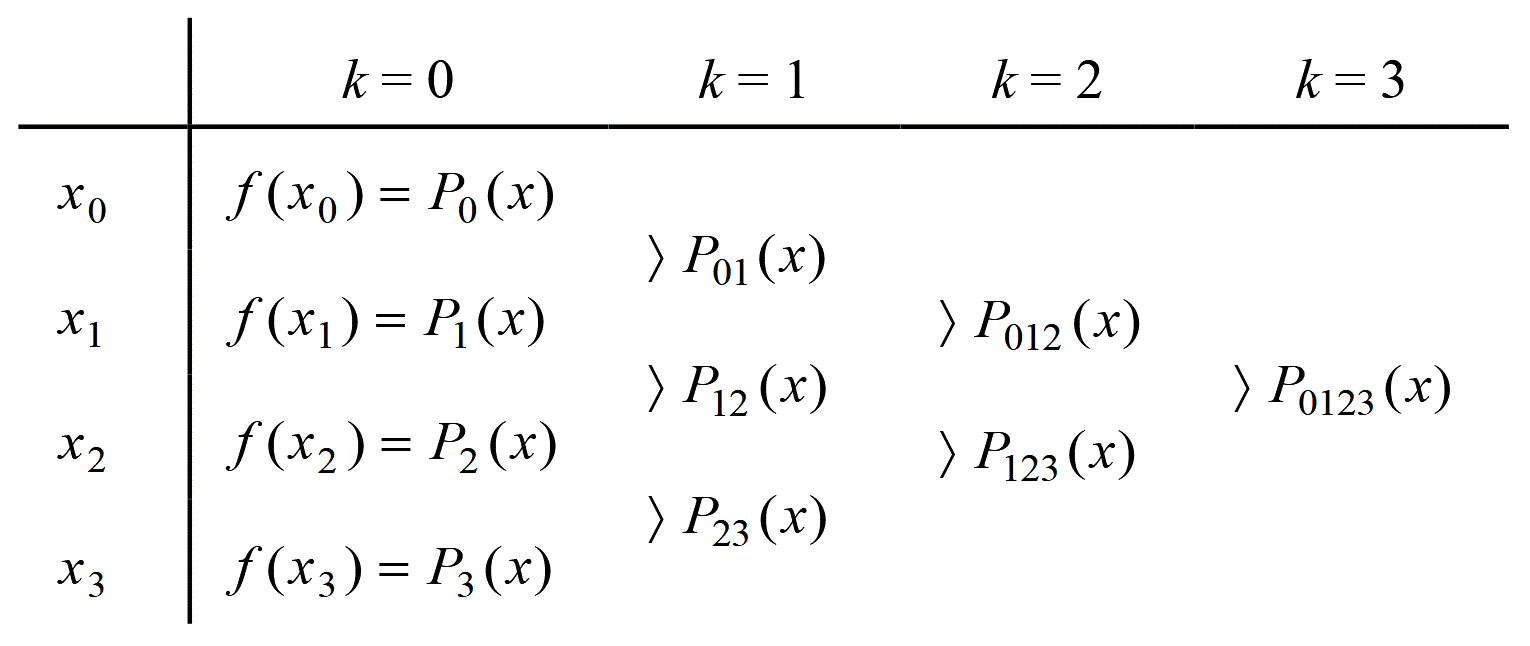
\includegraphics[scale = 0.28]{img/3/interpol_3_6}
\label{Ilustracja metody Neville'a}	
\end{figure}
%Rysunek 3.3: Ilustracja metody Neville'a
\end{frame}

\begin{frame}
$P_{1}, P_{2}, P_{3}, P_{4}$ -- wiel. stopnia $0$, przechodzący przez $(x_{i},\ f_{i})$ ,

$P_{12}, P_{23}, P_{34}$ -- wartość w $x$ dla wielomianów stopnia 1, przechodzącego przez pary punktów, \\
\vspace{4mm}
\textbf{Rekurencyjne zapełnianie tabeli:}
\begin{gather*}
	P_{i(i+1)\ldots(i+m)}(x)=\\
	=\displaystyle \frac{(x-x_{i+m})P_{i(i+1)\ldots(i+m-1)}(x)+(x_{i}-x)P_{(i+1)(i+2)\ldots(i+m)}(x)}{x_{i}-x_{i+m}}
\end{gather*}

\begin{itemize}
\item Otrzymamy wartości dla wielomianu stopnia $N-1$

\item zgodnego z $f(x)$ w węzłach, np.:
$$
P_{12}=\frac{(x-x_{2})P_{1}-(x-x_{1})P_{2}}{x_{1}-x_{2}}\ ;\ P_{12}(x_{1})=P_{1};P_{12}(x_{2})=P_{2}
$$

\end{itemize}

\end{frame}

%\begin{frame}


%Wygodniej-- różnice między pokoleniami:
%$$
%C_{m,i}=P_{i\cdots(i+m)}-P_{i\cdots(i+m-1)}\ ;\ %D_{m,i}=P_{i\cdots(i+m)}-P_{i\cdots(i+m)}
%$$
%$$
%D_{m+1,i}\ =\ \frac{x_{i+m+1}-x}{x_{i}-x_{i+m+1}}(C_{m,i+1}-D%_{m,i})
%$$
%$$
%C_{m+1,i}\ =\ \frac{x_{i}-x}{x_{i}-x_{i+m+1}}(C_{m,i+1}-D_{m,%i})
%$$
%\vspace{3mm}

%Końcowy wynik -- suma różnic wzdłuż wybranej ścieżki. \\
%Dodatkowo otrzymujemy oszacowanie błędu. \\
%\vspace{3mm}
%\textbf{Zadanie}: sprawdzić poprawność, napisać algorytm, \\
%oszacować błąd.
%\end{frame}

    %%%%%%%%%%%%%%%%%%%%%%%
    \section{Metoda ilorazów różnicowych (divided differences, Newtona)}
\begin{frame}
{3.7 Metoda ilorazów różnicowych (divided differences, Newtona)}

Interesuje nas nie wartość, a  postać wielomianu (dobra do celów praktycznych)

$P_{n}(x)-\text{LIP, stp. } \leq n$, zgodny z $f(x)$ w $\{x_{0},\ x_{1},\ .\ .\ .\ ,\ x_{n}\}$

Można go zapisać w postaci:
\begin{equation*}\begin{split}
P_{n}(x)=a_{0}+a_{1}(x-x_{0})+a_{2}(x-x_{0})(x-x_{1})+ \\
\cdots+a_{n}(x-x_{0})(x-x_{1})\cdots(x-x_{n-1})
\end{split}
\end{equation*}

$a_{0}$: $f(x_{0})=P_{n}(x_{0})=a_{0}$

$a_{1}$ : $f(x_{1})=P_{n}(x_{1})=a_{0}+a_{1}(x_{1}-x_{0})=f(x_{0})+a_{1}(x_{1}-x_{0}) \Rightarrow$

$$
a_{1}=\frac{f(x_{1})-f(x_{0})}{x_{1}-x_{0}}
$$
\end{frame}

\begin{frame}
Wprowadzamy notację:
\begin{itemize}
\item 0-wy iloraz różnicowy wzgl. $x_{i}$ : $f[x_{i}]=f(x_{i})$ \\
pozostałe - indukcyjnie:

\item 1-szy:
$$
f[x_{i},\ x_{i+1}]=\frac{f[x_{i+1}]-f[x_{i}]}{x_{i+1}-x_{i}}
$$
Gdy zaś określone są ilorazy aż do $(k-1)$ , czyli
$$
f[x_{i},\ x_{i+1},\ x_{i+k-1}] \: i \: f[x_{i+1},\ x_{i+2},\ x_{i+k}]
$$
\item to wtedy k-ty iloraz różnicowy:
\end{itemize}
$$
f[x_{i},\ x_{i+1}, ...\ x_{i+k}]=\frac{f[x_{i+1},x_{i+2},\ldots.x_{i+k}]-f[x_{i},x_{i+1},\ldots.x_{i+k-1}]}{x_{i+k}-x_{i}}
$$
\end{frame}
\begin{frame}{Budowa tablicy ilorazów różnicowych}
\begin{itemize}
    \item wystarczy zrobić tylko raz dla danego zestawu węzłów interpolacji
    \item do wzoru wykorzystujemy wyniki na przekątnej (czerwone)
    \item dodanie nowego węzła nie wymaga powtarzania obliczeń od początku
    
\end{itemize}

  \begin{array}{llllll} 
  x_0 & \color{red} f(x_0) \\ 
  x_1 & f(x_1) & \color{red}  f[x_0,x_1] \\ 
  x_2 & f(x_2) & f[x_1,x_2] & \color{red}  f[x_0,x_1,x_2] \\ 
  \ldots & \ldots & \ldots & \ldots & \ldots & \ldots\\ 
  x_n & f(x_n) & f[x_{n-1},x_n] & \ldots & \ldots & \color{red}  f[x_0,\ldots,x_n] 
  \end{array}
\end{frame}
\begin{frame}
Interpolacyjny wzór Newtona z ilorazami różnicowymi:
$$
 P_{n}(x)=
   f[x_{0}]+(x-x_0) f[x_{0}, x_{1}]+(x-x_0) (x-x_1)f[x_{0},x_{1},x_{2}]+ \\
+ \cdots +(x-x_{0})(x-x_{1})\cdots(x-x_{n-1})f[x_{0},x_{1},\dots ,x_{n}]
$$\\
$$
P_{n}(x)=f[x_{0}]+\sum_{k=1}^{n}f[x_{0},\ x_{1},\ .\ .\ .\ ,\ x_{k}](x-x_{0})\cdots(x-x_{k-1})
$$
Postać Newtona $\rightarrow$ do obliczania wartości wielomianu najlepiej użyć wariantu schematu Hornera
%\textbf{Zadanie}: Policzyć $a_{2}, a_{3}$, zapisać algorytm.

\end{frame}


\begin{frame}
Związek ilorazów różnicowych z pochodnymi.
\begin{block}
{Generalized Mean value theorem}

Założenia:
\begin{itemize}
\item $f\in C^{n}[a,\ b]$
\item $x_{0}, x_{1}$, . . . , $x_{n}\in[a,\ b] $ i są różne
\end{itemize}

Teza:
$$
\exists\eta\in(a,\ b)\ f[x_{0},\ x_{1},\ .\ .\ .\ ,\ x_{n}]=\frac{f^{(n)}(\eta)}{n!}
$$
\end{block}
\vspace{5mm}

\textbf{Materiały o potrzebnych twierdzeniach.} \url{https://tinyurl.com/tb95zoe}
\end{frame}

\begin{frame}
\textbf{Wzor Newtona dla węzłów równoodległych}

$h=x_{i+1}-x_{i} \quad i=0, 1, ..., n-1$ \\
$x_i=x_0+i\cdot h$\\
$x=x_{0}+s\cdot h$ \\
$x-x_{i}=(s-i)h$ \\

\begin{gather*} P_{n}(x)=P_{n}(x_{0}+s\cdot h) =\\
   f[x_{0}]+s\cdot h\cdot f[x_{0}, x_{1}]+s(s - 1)h^{2}f[x_{0},x_{1},x_{2}]+ \\
+ \cdots +s(s-1)\cdots(s-n+1)h^{n}f[x_{0},x_{1},\dots ,x_{n}]
\end{gather*}

\begin{gather*}
\binom{s}{k}=\displaystyle \frac{s(s-1)\ldots(s-k+1)}{k!}\\
P_{n}(x)=P_{n}(x_{0}+sh)=\sum_{k=0}^{n}(_{k}^{s})k!h^{k}f[x_{0}, x_{1}, \cdots ,x_{k}](**)
\end{gather*}
\end{frame}
\begin{frame}{Różnica progresywna(forward difference)}
Progresywna, bo pomiędzy $i$ oraz $i+1$ (do przodu):
  \begin{gather*}
    \Delta^{(0)} y_i := y_i\\
    \Delta^{(k)} y_i := \Delta^{(k - 1)} y_{i+1} - \Delta^{(k - 1)} y_i, k \ge 1
  \end{gather*}

  Forward differences -- przykład dla 4 punktów:
  \begin{figure}[h]
  			\includegraphics[width = 0.4 \linewidth]{img/3/interpol_3_7}
  	\end{figure}
\end{frame}
\begin{frame}{Newton forward divided-difference formula }
\begin{itemize}
\item Dla węzłów równoodległych iloraz różnicowy jest równy:
$$f[x_{0},\displaystyle \ x_{1},\cdots,\ x_{k}]=\frac{1}{k!h^{k}}\triangle^{k}f(x_{0})$$ \\

\item Podstawiając do (**) mamy:
$$P_{n}(x)=P_n(x_0+s\cdot h)=\displaystyle
\sum_{k=0}^{n}(_{k}^{s})\triangle^{k}f(x_{0})$$
\item Dysponując wartościami różnic progresywnych można wyznaczyć wartość wielomianu.
\end{itemize}
\end{frame}



    %%%%%%%%%%%%%%%%%%%%%%%
    \section{Interpolacja Hermite'a}
%\begin{frame}
%{3.8 Interpolacja Hermite'a}

%Więcej o metodzie i jej autorze \\
%(autor: Shayne Waldrom,University of Auckland):\\
%\vspace{5mm}
%https://www.math.auckland.ac.nz/$\sim$waldron/Hermite/he%rmite.html
%\end{frame}

%
\begin{frame}{Interpolacja Hermite'a}
\textcolor{blue}{Dane:}
\begin{itemize}
\item $k+1$ różnych węzłów: $x_{0}, x_{1}, \dots, x_{k}$

\item tzw. krotności węzłów dane liczbami naturalnymi $m_{0}, m_{1},\dots , m_{k}, \displaystyle \sum_{i=0}^{k}m_{i}=n+1$
\end{itemize}
\textcolor{blue}{Szukamy:}

Dla dowolnej funkcji $f$ -- szukamy wielomianu $H_{n}$ stopnia $\leq n,$ \\
takiego, że:

$H_{n}^{(j)}(x_{i})=f^{(j)}(x_{i})$ \quad dla $i=0, 1, \dots , k$ oraz
$j=0, 1, \dots, m_{i}$\\
\vspace{0.5cm}
Krotność mówi nam, ile pochodnych ma być równych.
Gdy $m_{i}=1$ -- interpolacja Lagrange'a.
\end{frame}

\begin{frame}{Rozwiązanie}
Suma krotności $i$ początkowych węzłów interpolacyjnych
\vspace{2mm}
$s(i)=\left\{\begin{array}{l}
0,\ i=0\\
m_{0}+m_{1}+\cdots+m_{i-1},\ i>0
\end{array}\right.$
\vspace{2mm}\\

Zauważmy, że każda liczba 
$0\leq l\leq n$ da się przedstawić w postaci $l=s(i)+j$ gdzie $0 \leq i \leq k$ oraz $0 \leq j \leq m_{i}-1$\\
\vspace{0.5cm}
Definiujemy wielomiany:\\
$p_{s(0)}(x)=1$

$p_{(s(i)+j)}(x)=(x-x_{0})^{m_{0}}(x-x_{1})^{m_{1}}\ldots(x-x_{i-1})^{m_{i-1}}(x-x_{i})^{j}(\star)$ \\
gdzie: $i=0, 1, \dots, k; \: j=0, 2, \dots , m_{i}-1$ \\
Wtedy szukany wielomian interpolacyjny to kombinacja linowa takich wielomianów (por. postać Newtona)
$$
H_{n}(x)=\sum_{l=0}^{n}b_{l}\cdot p_{l}(x)=\sum_{i=0}^{k}\sum_{j=0}^{m_{i-1}}b_{(s(i)+j)}\cdot p_{(s(i)+j)}(x)
$$
\end{frame}

\begin{frame}
Jak znaleźć współczynniki $b_{l}$:

$l$ - ustalone, $l=s(i)+j$
$$
H_{n}(x)=\underbrace{A(x)}_{b_{0},{b_{1},\ldots,b}_{l-1}}+b_{l}p_{l}(x)+\underbrace{B(..x)}_{b_{l+1},\ldots,b_{n}}(\star\star)
$$
gdzie:
$A(x)$ - kombinacja liniowa wielomianów $b_i$ o znanych już współczynnikach $b_{0},{b_{1},\ldots,b}_{l-1}$\\

\vspace{3mm}
$B(x)$ - kombinacja liniowa wielomianów $b_i$ o współczynnikach $b_{l+1},\ldots,b_{n}$
\end{frame}
\begin{frame}
Biorąc pod uwagę (*)
$$
p_{l}(x)=p_{(s(i)+j)}(x)=p_{s(i)}(x)(x-x_{i})^{j}
$$
oraz dla $m > l$ czyli wielomianów wchodzących w skład $B(x)$, każdy jest postaci
$$
p_{m}(x)=f_m(x)*(x-x_{i})^{k}(***)
$$
gdzie $k>j$ oraz $f_m(x)$ zawiera czynniki z(*) dla pozostałych węzłow. \\
\end{frame}
\begin{frame}
różniczkując $(\star\star)$ korzystamy ze wzoru na pochodną iloczynu 

$$
(f\cdot g)^{(j)}=f^{(j)}\cdot g+ {n\choose 1} f^{(j-1)}\cdot g^{(1)}+{n\choose 2} f^{(j-2)}\cdot g^{(2)}+f\cdot g^{(j)}
$$
oraz faktu, że dla $j\leq k$
$$
((x-x_i)^{k})^{(j)}=k\cdot (k-1) ...(k-j+1)(x-x_i)^{k-j}
$$
Interesuje nas $H_{n}^{(j)}(x_{i})$\\
Ze względu na (***) $B^{(j)}(x_i)=0$ i mamy:
$$
H_{n}^{(j)}(x_{i})=A^{(j)}(x_{i})+b_{l}p_{s(i)}(x_{i})j!
$$
korzystając $\mathrm{z}$:
$$
H_{n}^{(j)}(x_{i})=f^{(j)}(x_{i})
$$
mamy:
$$
b_{l}=\frac{f^{(j)}(x_{i})-A^{(j)}(x_{i})}{p_{s(i)}(x_{i})j!}
$$

\end{frame}

    %%%%%%%%%%%%%%%%%%%%%%%
    \section{Efekt Rungego}
\begin{frame}
{3.9 Efekt Rungego}

\begin{block}{}
	\textbf{Intuicja: } Zwiększenie liczby węzłów $\Rightarrow$ lepsza dokładność. \\
	\textbf{Rzeczywistość: } Efekt Rungego -- zmniejszenie dokładności.
\end{block}

(C. Runge, 1901)
$$
y(x)=\frac{1}{1+25x^{2}},\ x\in[-1,\ 1]
$$
Występuje, gdy:
\begin{itemize}
\item interpolujemy wielomianami

\item węzły interpolacyjne są równoodległe
\end{itemize}
\end{frame}

\begin{frame}
	\begin{figure}[h]
		\includegraphics[scale=0.35]{img/3/interpol_3_9}
	\end{figure}
\end{frame}

\begin{frame}
\begin{itemize}
\item Katastrofalna rozbieżność dla $0.726\leq|x|<1$.

\item Lecz bardzo dobra zbieżność w strefie centralnej.
\end{itemize}

(Konsekwencja tego, że zadanie to jest {\itźle uwarunkowane}.)
\vspace{0.5cm}

Efekt Rungego -- rady praktyczne:

\begin{itemize}
\item zaczynać od interpolacji liniowej,

\item zwiększać liczbę węzłów i stopień wielomianu, aż do ustabilizowania istotnych miejsc.
\end{itemize}
\vspace{0.5cm}
Inne sposoby:
\begin{itemize}
\item interpolacja funkcjami sklejanymi
\item specjalny dobór węzłów.
\end{itemize}

\end{frame}





\end{document}
